\section{Signal and background modelling}
\label{chp:sec:sigbkg}

The topologies of the signals searched in this dissertation make $t\bar{t}+$jets production the main background for the analyses. In particular, $t\bar{t}+\ge1 b$ is the main irreducible background in the signal regions. Other background contributions arise from single top-quark production, from the production of a single $W$ or $Z$ boson in association with jets ($W$/$Z$+jets), diboson production in association with jets ($WW$, $WZ$ and $ZZ$ + jets), as well as from the associated production of a vector boson $V$ ($V$ = $W$, $Z$, $\gamma^{*}$) and a $t\bar{t}$ pair ($t\bar{t}V$). Multijet events contribute to the lepton+jets sample via the misidentification of a jet or a photon as an electron, or the presence of a non-prompt lepton, e.g. from a semileptonic $b$- or $c$-hadron decay; in contrast, they enter the all-hadronic$+$\MET sample via instrumental effects such as jet energy mismeasurements that contribute to \MET. All backgrounds are estimated using samples of simulated events that are initially normalised to their theoretical cross sections, with the exception of the multijet background, which is estimated using data-driven methods in the lepton+jets sample.\par
The top-quark mass and the Higgs boson mass are set to 172.5 $\gev$ and 125 $\gev$ respectively in all simulated samples. Unless stated otherwise, in the following the accuracy of the calculation indicated for all samples corresponds to the order in the strong coupling constant at which the matrix element is computed. All simulated samples use {\sc Photos} for photon radiation, {\sc Tauola} for $\tau$ decays and {\sc EvtGen} (except for the samples simulated by {\sc Sherpa}) for decays of $b$- and $c$-hadrons.
Simulated samples also include contributions from pileup and UE and are processed through a full simulation of the detector geometry and response using {\sc Geant4}, with the exception of the signal samples of associated heavy-Higgs production, for which the AF2 simulation was used. All event generators using {\sc Herwig} are also interfaced to {\sc Jimmy} to simulate the UE. All simulated samples are processed through the same reconstruction software as the data. Simulated events are corrected so that the object identification efficiencies, energy scales and energy resolutions match those determined in data control samples. 


\subsection[$t\bar{t}$+jets production]{\boldmath{$t\bar{t}$}+jets production}
\label{chp:data:sec:ttbar}
The large phase space covered by the analyses discussed in this dissertation requires a $t\bar{t}$ simulation that describes correctly the different event topologies, especially the emission of additional jets and the heavy-flavour fraction. Not only the normalisation, but also the kinematics of the full final state have to be correctly modelled since several kinematic variables are used. 

The  $t\bar{t}$   background is generated using the {\sc Powheg-Box} v2 NLO generator with the CT10 PDF set, which has been chosen as the baseline generator for the modelling of $t\bar{t}$  production based on measurements at $\sqrt{s}=7$ and 8 $\tev$ \cite{Aaboud:2016iot,Aad:2014zka,Aad:2015mbv}. The {\tt hdamp} parameter, which controls the $\pt$ of the first additional emission beyond the Born configuration, is set equal to the top-quark mass. The parton shower and hadronisation are modelled by {\sc Pythia} 6.428 with the CTEQ6L1 PDF set \cite{Pumplin:2002vw} and the Perugia2012 \cite{perugia} settings for the tunable parameters of the underlying event (UE tune). The
sample is normalised to the {\sc Top++} 2.0 \cite{topPP} theoretical cross section of $832^{+46}_{-51}$ pb, calculated at next-to-next-to-leading order (NNLO) in QCD and including resummation of next-to-next-to-leading logarithmic (NNLL) soft-gluon terms \cite{Czakon:2012pz,Czakon:2012zr,Baernreuther:2012ws,Cacciari:2011hy}.

The $t\bar{t}$+jets sample is generated inclusively and events are categorised according to the flavour of additional jets in the event, using the following procedure. Particle jets are reconstructed from stable particles (excluding muons and neutrinos) using the anti-$k_{\rm T}$ algorithm with a radius parameter $R = 0.4$, and are required to have $\pt > 15$ $\gev$ and $|\eta| < 2.5$. The $\pt$ threshold for particle jets (15 \gev) is chosen to be 10 $\gev$ below the reconstructed-jet threshold, in order to allow for resolution effects. The flavour of the jets is determined by matching them within $\Delta R < 0.4$ to $b$- or $c$-hadrons. Jets matched to exactly one $b$-hadron with $\pt$ above 5 \gev, are labelled $b$-jets, while those matched to two or more $b$-hadrons are labelled $B$-jets (with no $\pt$ requirement on the second hadron); $c$- and $C$- jets are defined analogously, considering only jets not already defined as $b$- or $B$- jets. Events that have at least one $b$- or $B$-jet, not counting heavy-flavour jets from top-quark or $W$-boson decays, are labelled $t\bar{t}+\ge1b$, those with no $b$- or $B$-jet but at least one $c$- or $C$-jet are labelled $t\bar{t}+\ge1c$, while those with no heavy flavour jets are labelled $t\bar{t}+$light-jets. The $t\bar{t}+\ge1b$ and $t\bar{t}+\ge1c$ contributions are together referred to as $t\bar{t}$+HF, with HF denoting heavy flavour. 
In order to perform more detailed studies of the  $t\bar{t}$+HF modelling and the related systematic uncertainties, a more detailed categorisation is also used: events with at least three $b$- or $B$-jets are labeled $t\bar{t}+\ge3b$, those with exactly two $b$-jets are labelled $t\bar{t}+b\bar{b}$, those with only one $B$-jet are labelled $t\bar{t}+B$, and those with only one $b$-jet are labelled $t\bar{t}+b$; $t\bar{t}+\ge1c$ events are divided analogously. 

In the following sections some corrections applied to this simulation in order to improve its prediction are described.

\subsubsection[$t\bar{t}$+light-jets]{\boldmath{$t\bar{t}$}+light-jets}
The high $\ttbar$ production cross section and high-luminosity $pp$ collisions make the LHC a top-quark factory that allows precision measurements of the kinematics of the top quark compared to the Tevatron \cite{Cacciari:2011hy}. Detailed studies of a number of differential distributions of the top quarks in $t\bar{t}$ events using the $\sqrt{s}=7$, 8 and 13 $\tev$ datasets by the ATLAS detector \cite{Aaboud:2016iot,Aad:2014zka,Aad:2015mbv,Aaboud:2016syx,ATLAS-CONF-2016-040} revealed significant differences between the unfolded data distributions and the predictions from {\sc Powheg-Box+Pythia}. The most significant discrepancy with data is observed in the top-quark $\pt$ spectrum  where MC predictions tend to be harder than data, as shown in figures \ref {fig:dat:ttl:8tev} and \ref{fig:dat:ttl:13tev}.

\begin{figure}[h!]
\begin{subfigure}{0.5\textwidth}
  \centering
  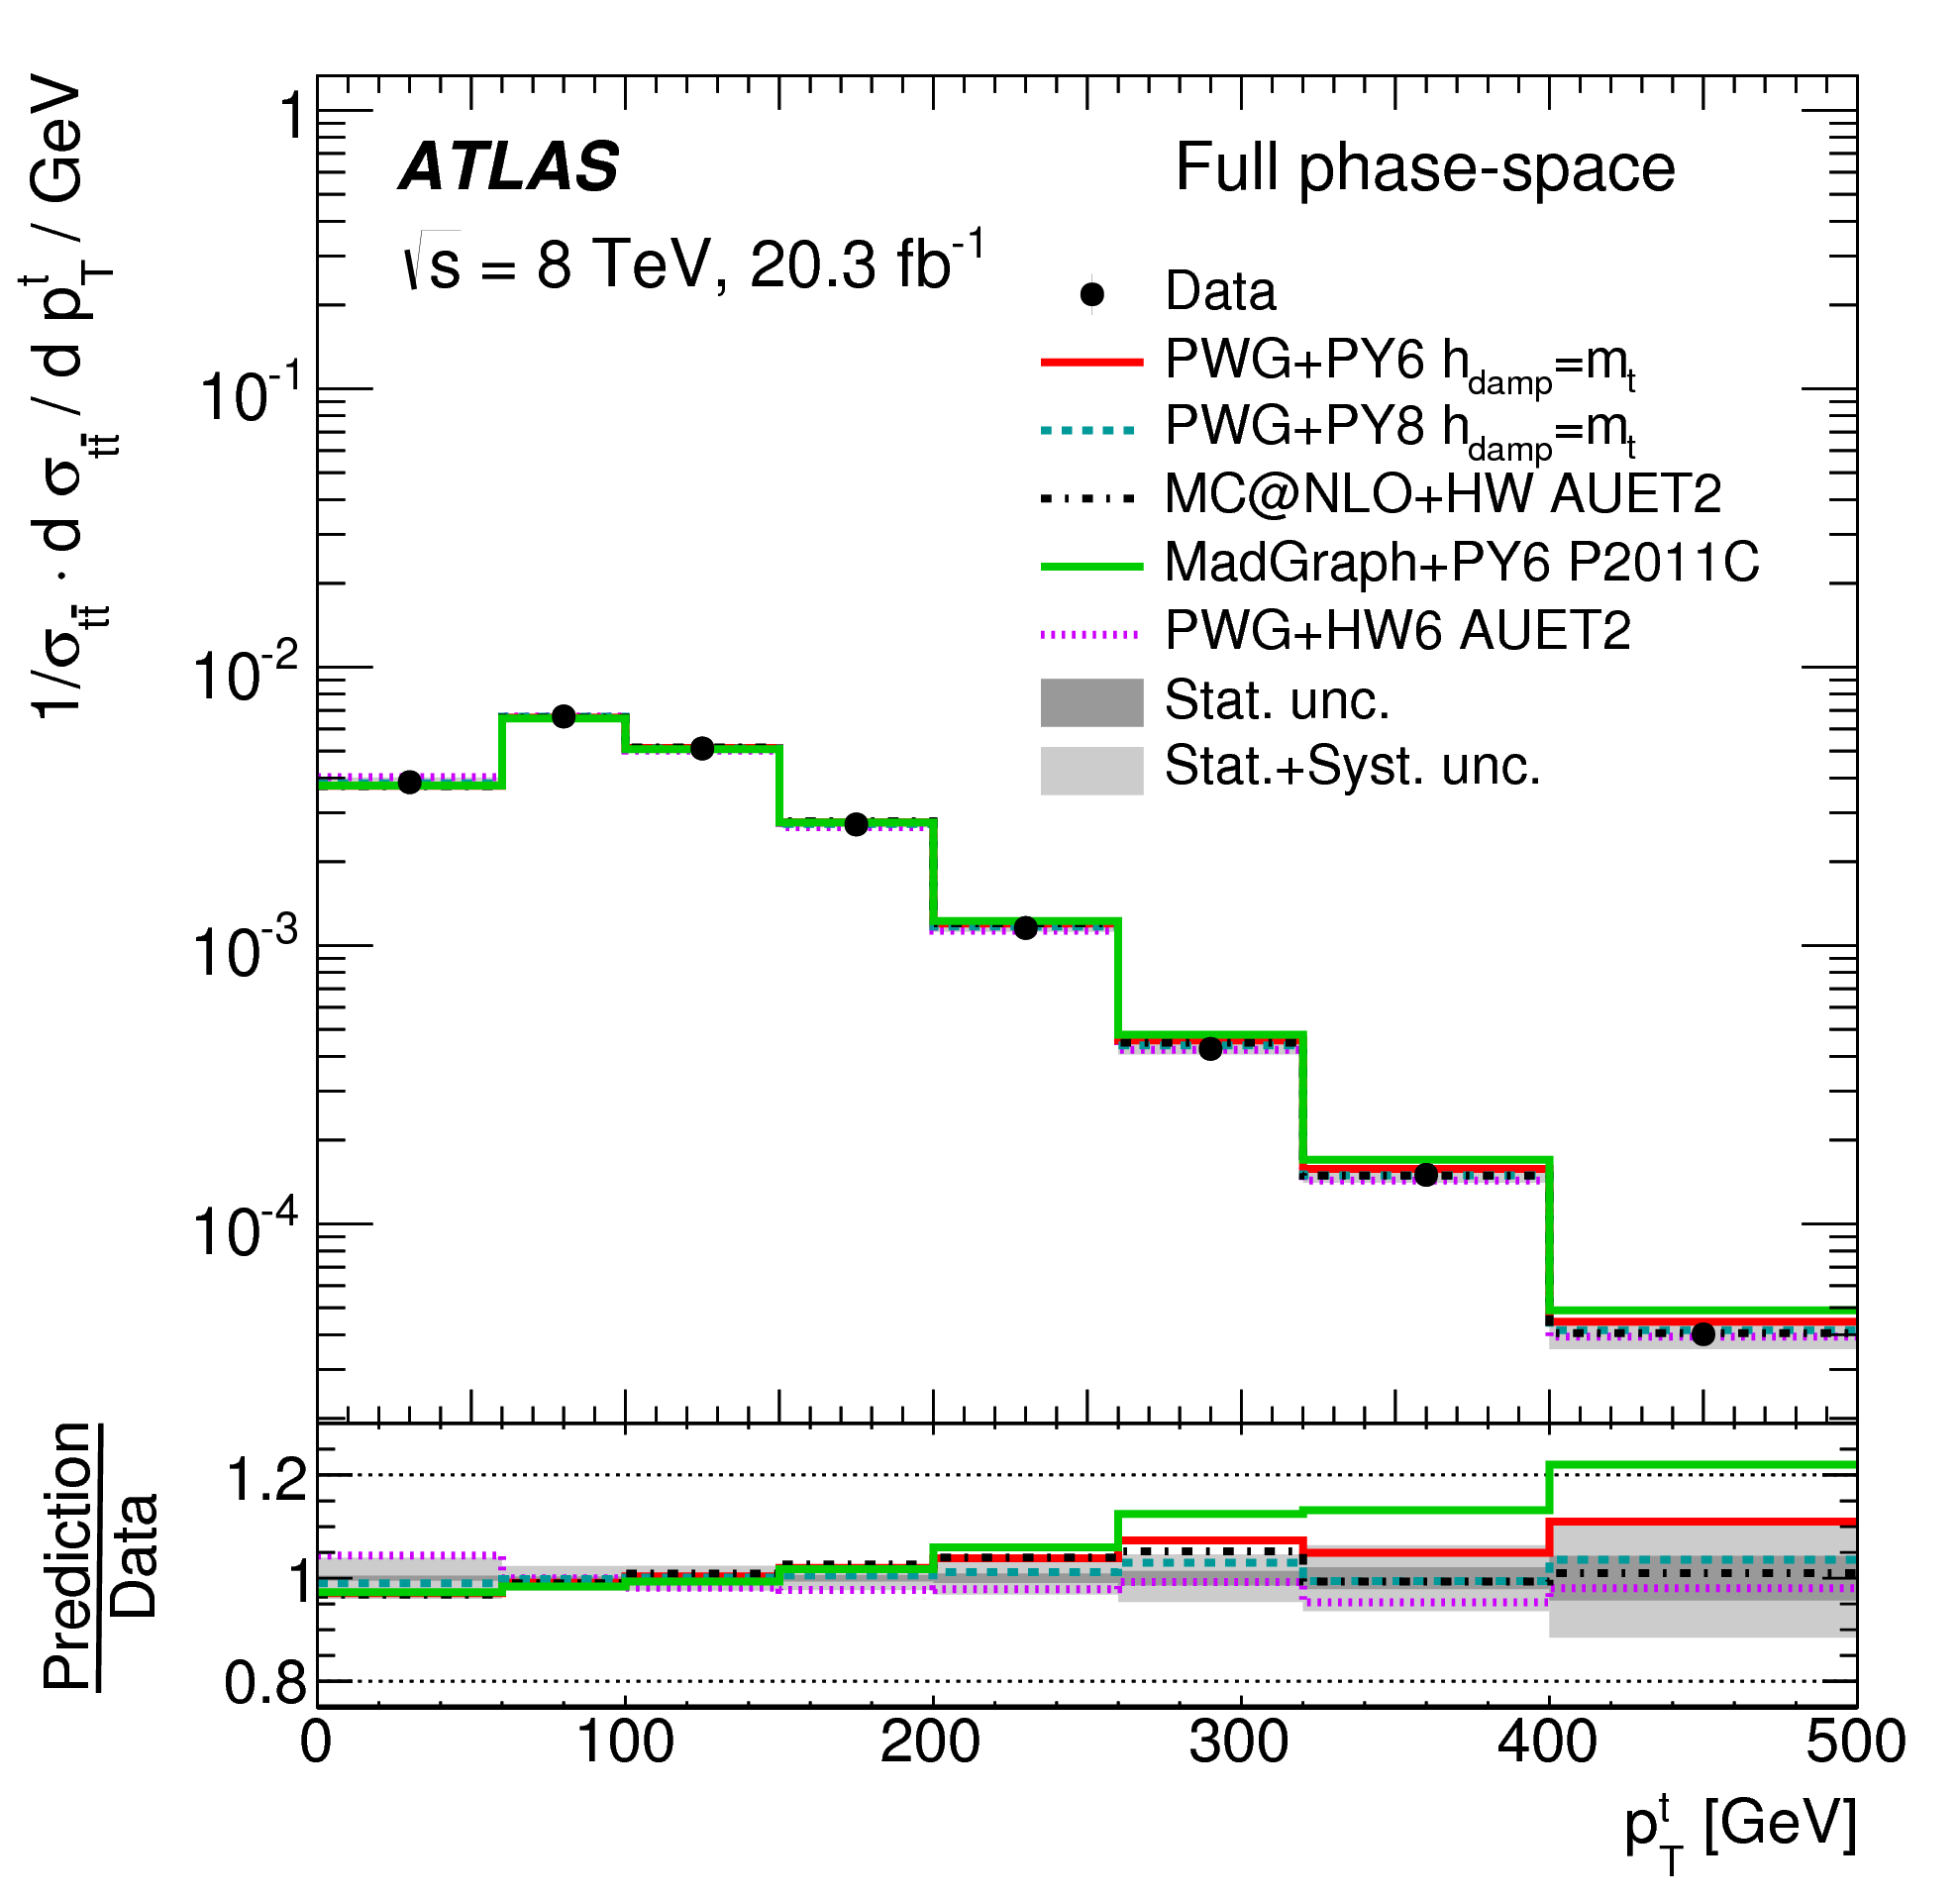
\includegraphics[width=0.9\textwidth]{figures/Datasamples/topptatlas.png}
  \caption{}
  \label{fig:dat:ttl:top}
\end{subfigure}
\begin{subfigure}{0.5\textwidth}
  \centering
  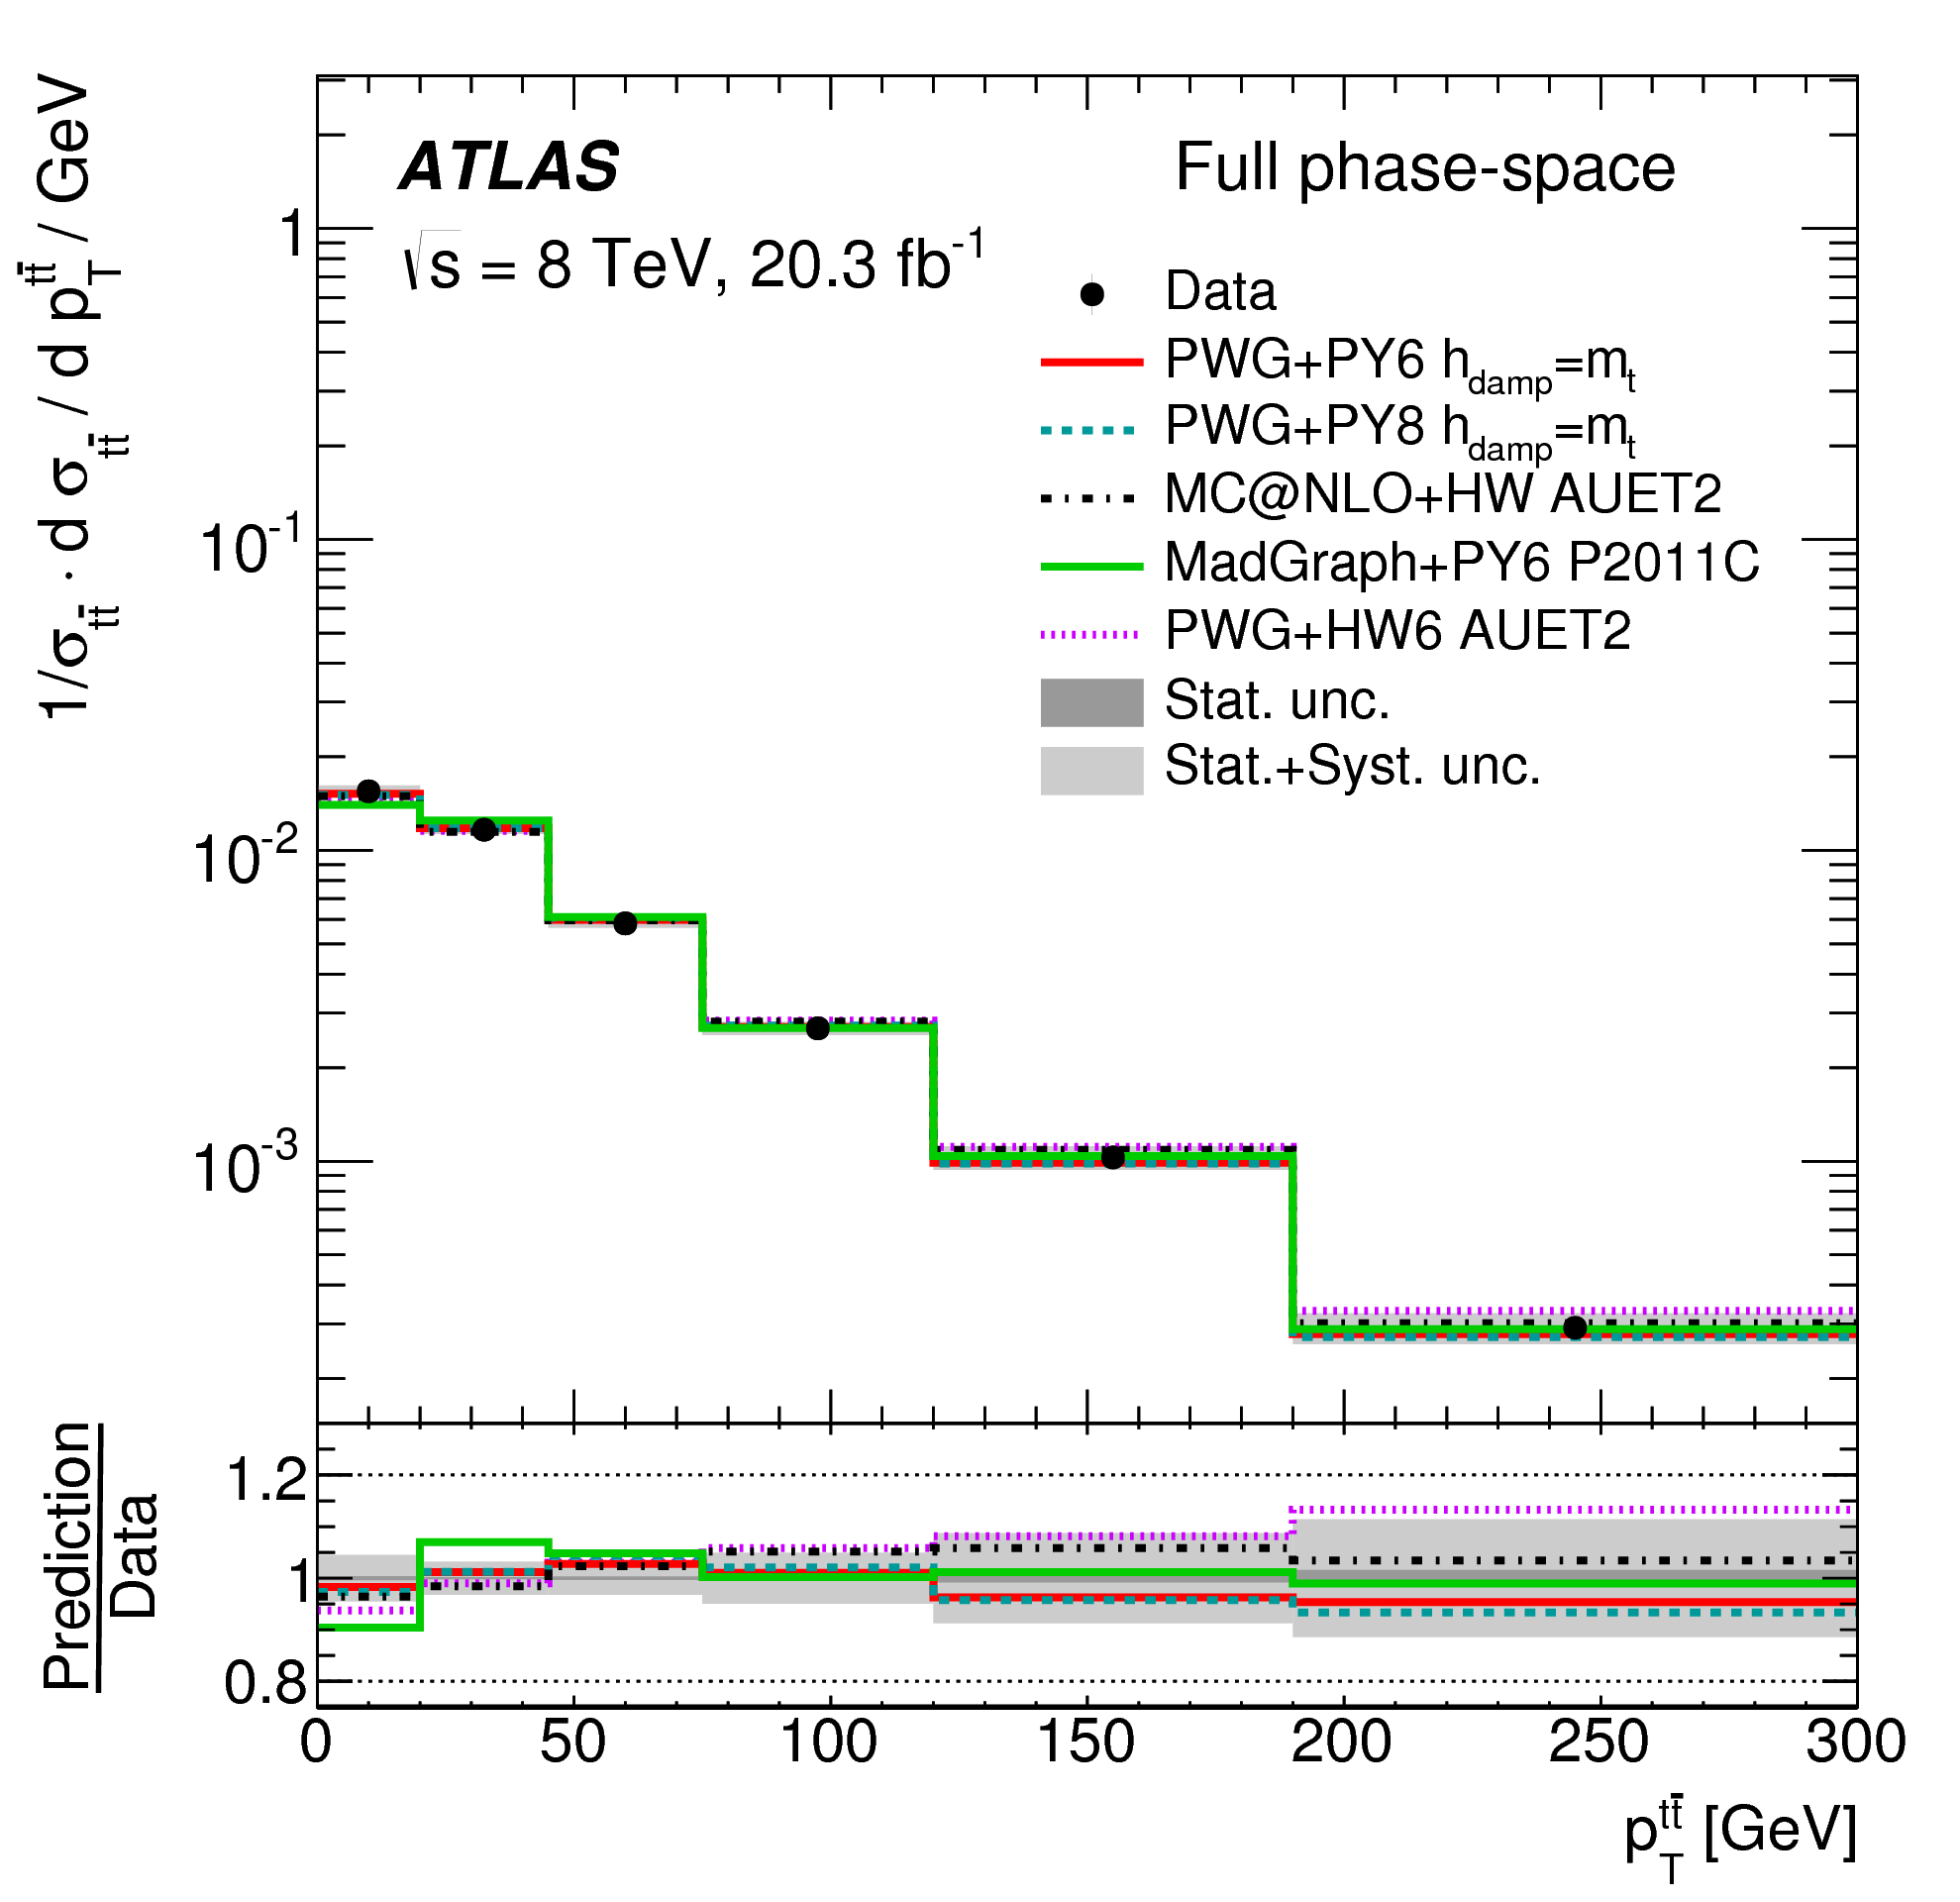
\includegraphics[width=0.9\textwidth]{figures/Datasamples/ttbarptatlas.png}
  \caption{}
  \label{fig:dat:ttl:ttbar}
\end{subfigure}

\captionsetup{width=0.85\textwidth} \caption{\small Normalised differential cross sections at 8 $\tev$ for (a) the transverse momentum of the hadronically-decaying top quark, $\pt^{\rm top}$, and (b) the transverse momentum of the $t\bar{t}$ system, $\pt^{t\bar{t}}$. The {\sc Powheg-Box+Pythia} prediction is shown in red. The gray bands indicate the total uncertainty on the data in each bin. From reference \cite{Aad:2015mbv}.}
\label{fig:dat:ttl:8tev}
\end{figure}

\begin{figure}[h!]
\begin{subfigure}{0.5\textwidth}
  \centering
  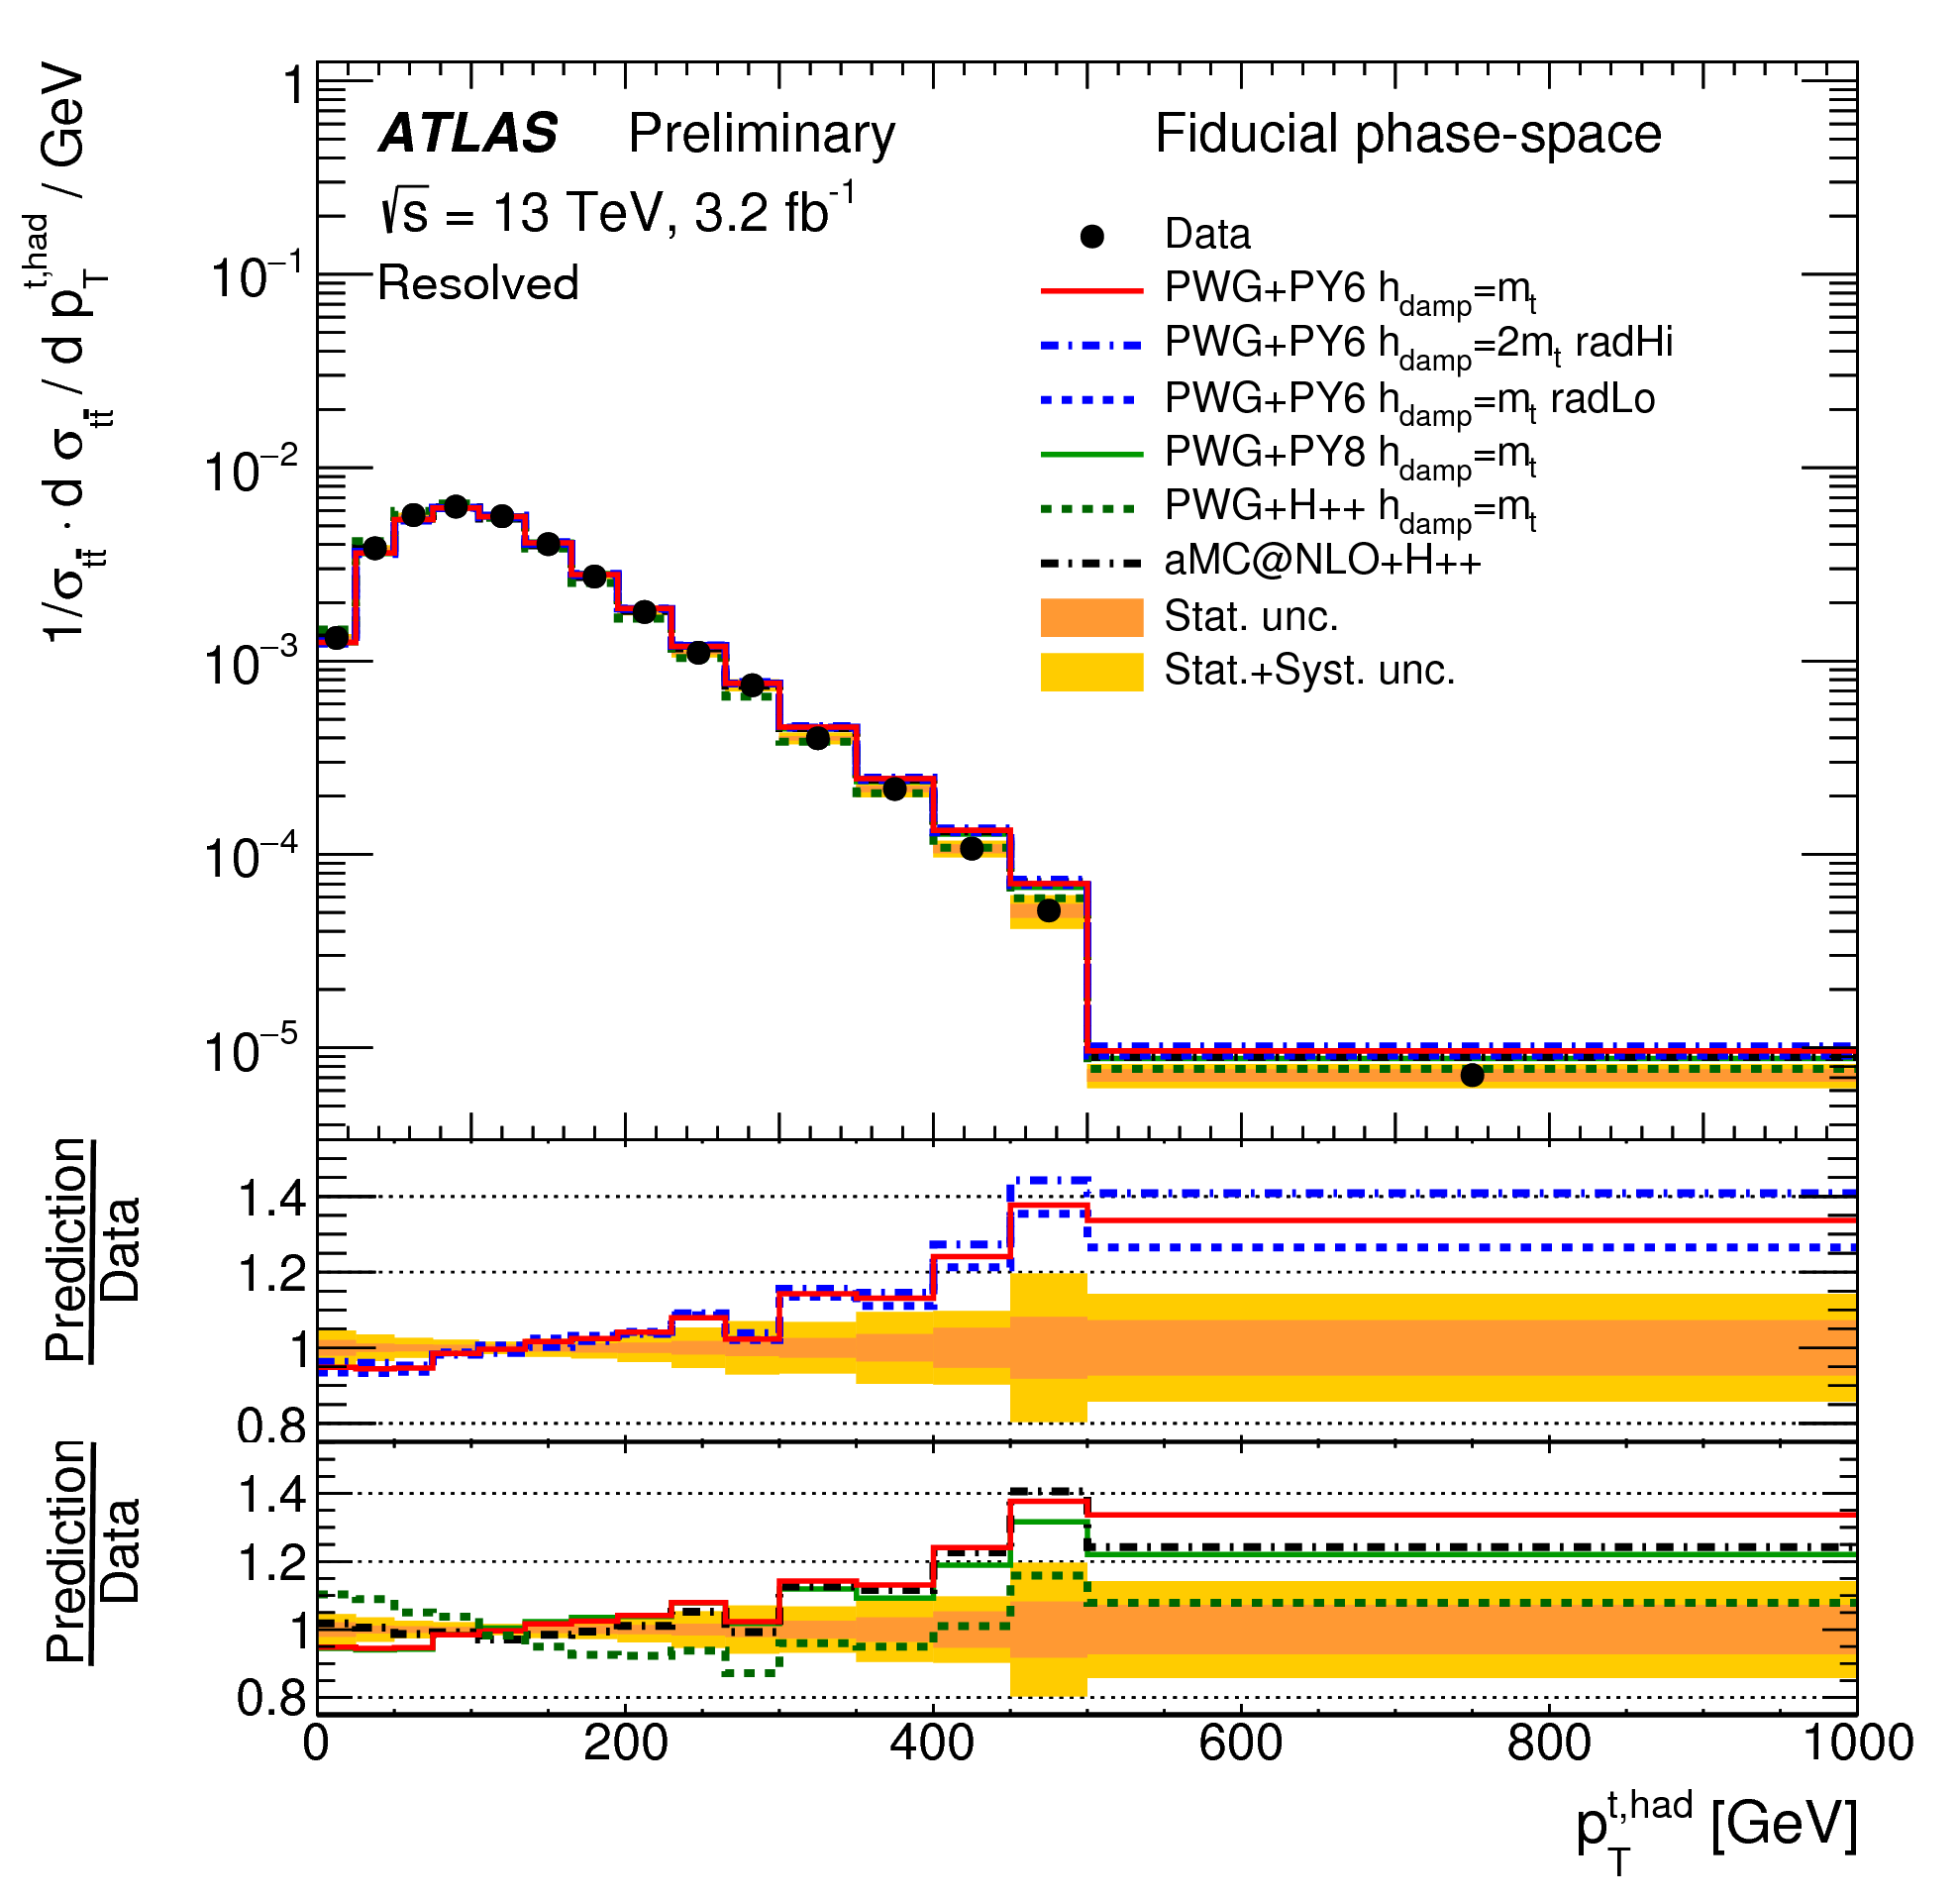
\includegraphics[width=0.9\textwidth]{figures/Datasamples/topptatlas13tev.png}
  \caption{}
  \label{fig:dat:ttl:top13}
\end{subfigure}
\begin{subfigure}{0.5\textwidth}
  \centering
  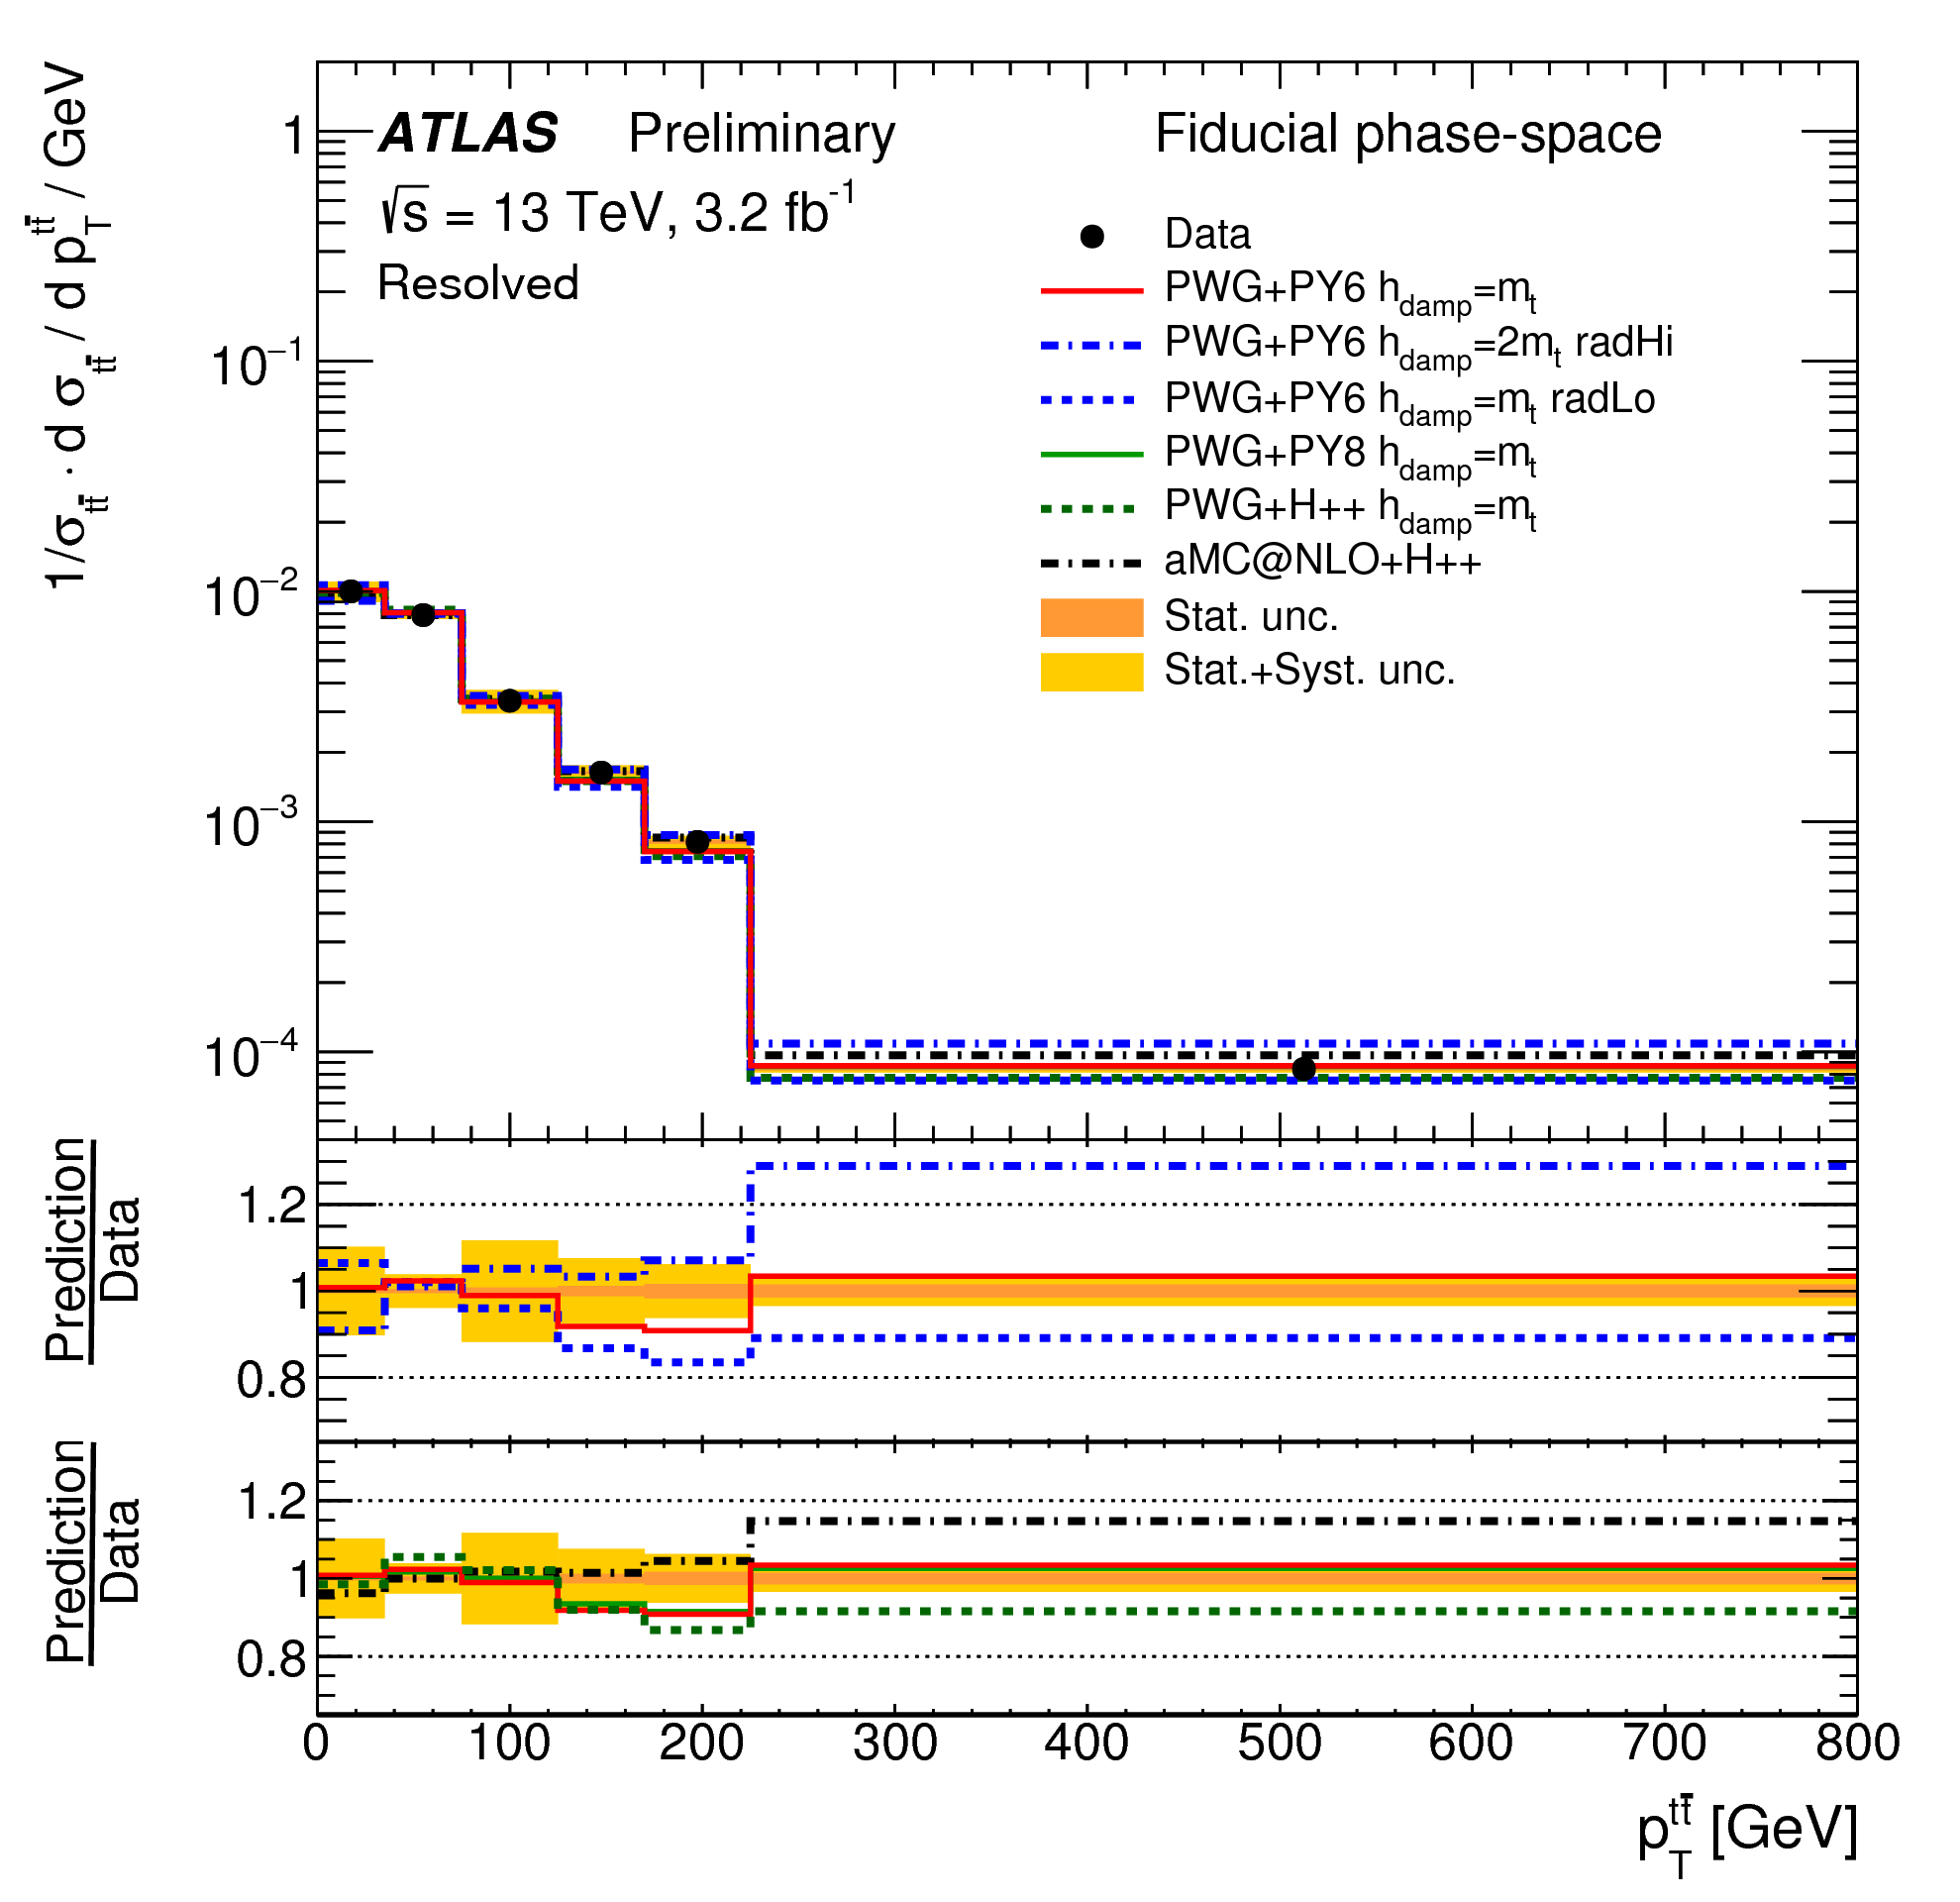
\includegraphics[width=0.9\textwidth]{figures/Datasamples/ttbarptatlas13tev.png}
  \caption{}
  \label{fig:dat:ttl:ttbar13}
\end{subfigure}

\captionsetup{width=0.85\textwidth} \caption{\small Normalised differential cross sections in the fiducial phase space at 13 $\tev$ for (a) the transverse momentum of the hadronically-decaying top quark, $\pt^{\rm top}$, and (b) the transverse momentum of the $t\bar{t}$ system, $\pt^{t\bar{t}}$. The {\sc Powheg-Box+Pythia} prediction is shown in red. The yellow bands indicate the total uncertainty on the data in each bin. From reference \cite{ATLAS-CONF-2016-040}.}
\label{fig:dat:ttl:13tev}
\end{figure}




A recent study \cite{PhysRevD.90.014006,Guzzi:2014wia} showed that missing higher-order QCD corrections to $\ttbar$ production can at least partly explain the ``top-quark $\pt$ discrepancy''. The NNLO QCD correction to the top-quark $\pt$ softens the spectrum and brings it closer to the $\sqrt{s}=8$ $\tev$ data, as shown in figure \ref{fig:dat:ttl:nnlo}.
\bfig[h!]
\centering
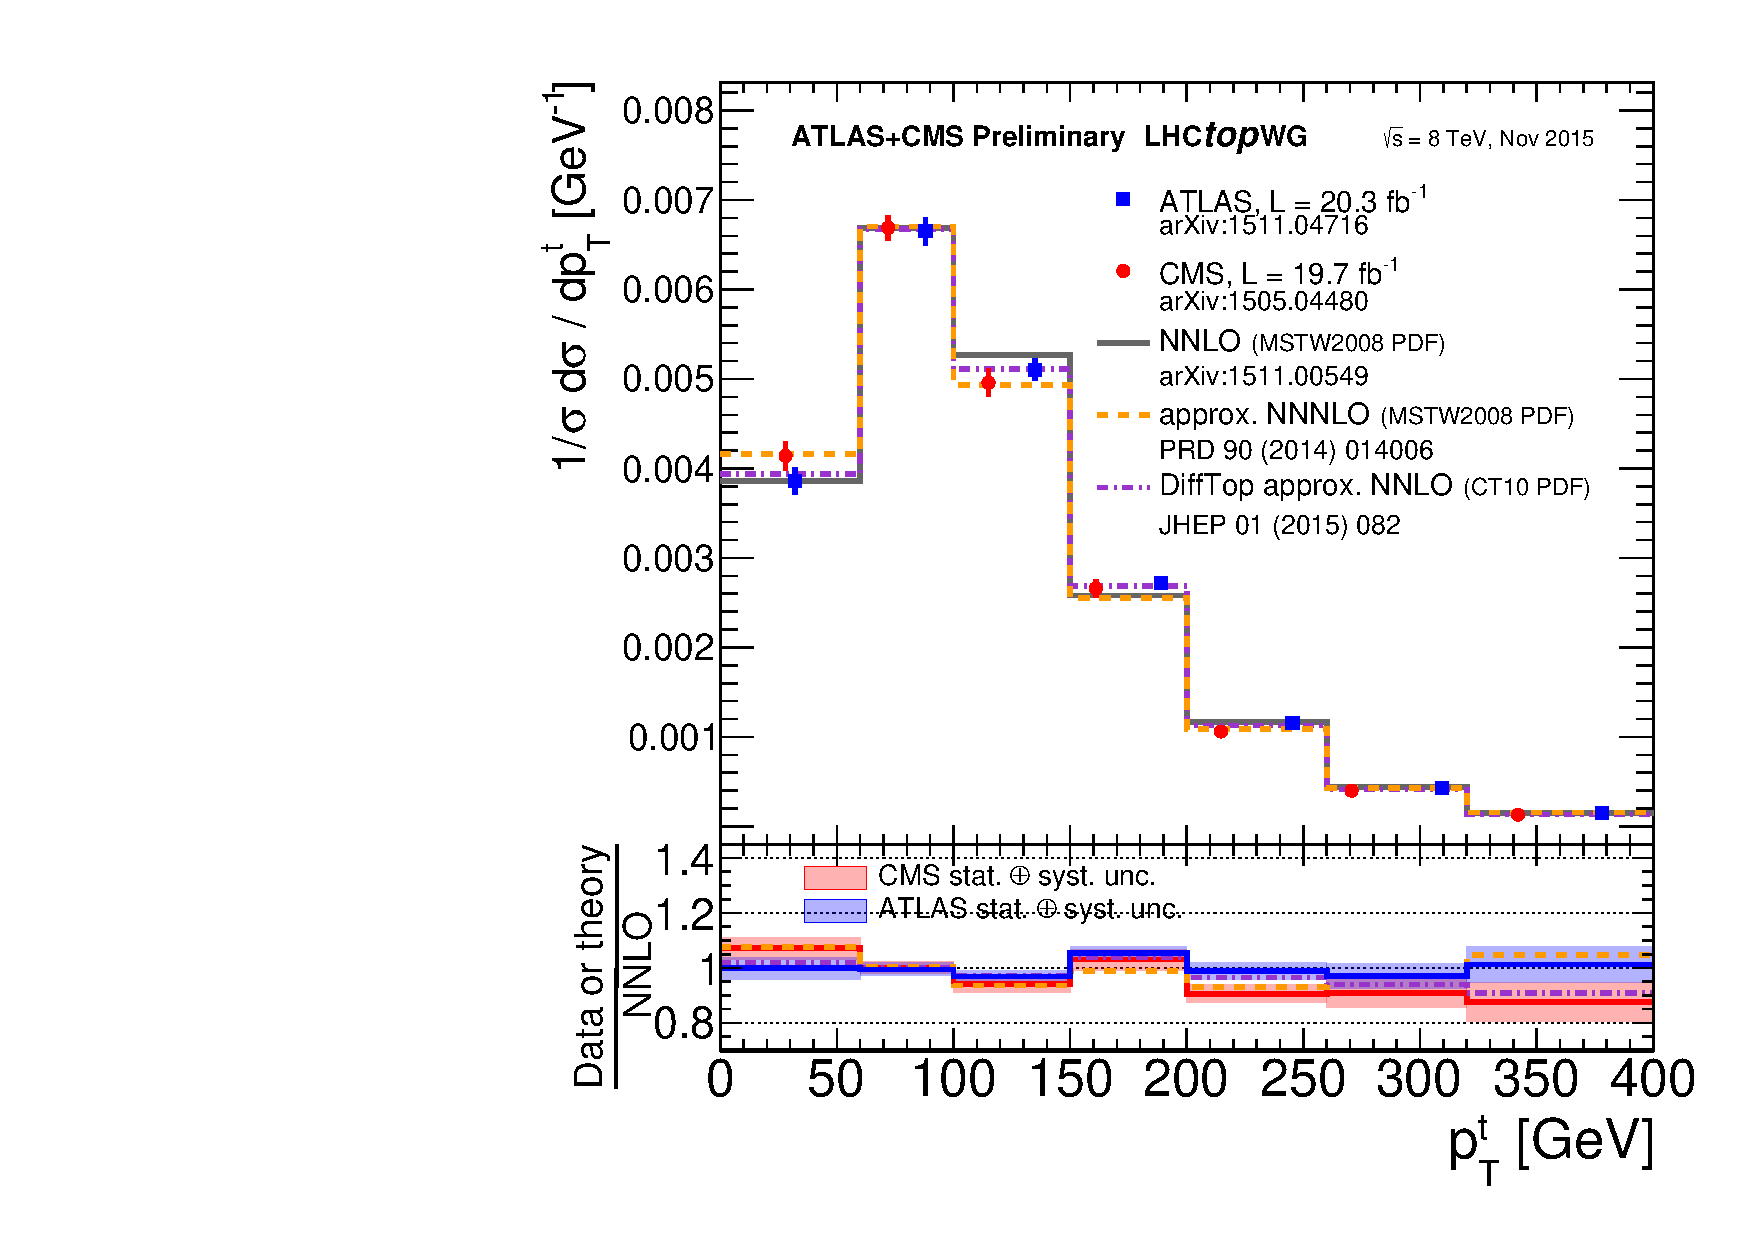
\includegraphics[width=0.5\textwidth]{figures/Datasamples/nnlo8tev.png}
\captionsetup{width=0.85\textwidth} \caption{\small Normalised differential cross section at 8 $\tev$ for the transverse momentum of the hadronically-decaying top quark, $\pt^{\rm top}$. The measurements from the ATLAS and CMS Collaborations are compared to different theoretical predictions.}
\label{fig:dat:ttl:nnlo}
\efig
To correct for this effect, two reweighting factors are derived from the NNLO calculation at $\sqrt{s}=13$ $\tev$ and their product is applied as a multiplicative factor to each event based on the value of top-quark $\pt$ and $t\bar{t}$-system $\pt$. First a reweighting factor based on $\pt^{t\bar{t}}$ is derived, in order to bring the $\pt^{t\bar{t}}$ distribution in {\sc Powheg-Box+Pythia} in agreement with the NNLO calculation. After applying this first reweighting factor, a second factor is derived to correct the $\pt^{\rm top}$ distribution. This two-step sequential procedure is needed in order to take into account the non-negligible correlation between both variables. Table \ref{tab:dat:ttl:PPfactors} summarises the correction factors. An alternative procedure, where only the $\pt^{\rm top}$ distribution is corrected, is available.
\begin{table}[bt!]\footnotesize
\centering
 
\begin{tabular}{ c c c c c c}
\hline
\hline
\multicolumn{6}{c}{ $\pt^{t\bar{t}}$}  \\
\hline
Bins [\gev]                 &    [0, 35]                 &   [35, 80]             &  [80, 140]             &  [140, 200] & [200,500)        \\
Rew. factor & 0.96 &  1.03 &  1.01 & 1.06 & 1.05  \\
\hline
\hline
\end{tabular}
\bigskip
 \makebox[\textwidth][c]{
\begin{tabular}{ c c c c c c c c c c}
\hline
\hline
\multicolumn{10}{c}{$\pt^{\rm top}$ }  \\
\hline
Bins [\gev]                 &    [0, 45]                   &   [45, 90]               &  [90, 135]              &  [135, 180]             &  [180, 225]              &  [225, 270]               &  [270, 315] & [315,400] & [400,800) \\
Rew. factor &   1.07 &  1.03 &  1.00  &  0.97  &  0.95  &  0.94  &  0.92 &  0.90 &  0.84   \\
\hline
\hline
\end{tabular}
}
 
\captionsetup{width=0.85\textwidth} \caption{\small Reweighting factors for the \textsc{PowHeg+Pythia} sample as a function of the $t\bar{t}$-system $\pt$ (top) and the top-quark $\pt$ (bottom). The two factors are multiplied to obtain the event weight correction.}
\label{tab:dat:ttl:PPfactors}
\end{table}
This reweighting procedure, which will be referred to as ``$t\bar{t}$ and top-quark $\pt$ reweighting'', is applied inclusively to two subsamples: $t\bar{t}+$light-jets and $t\bar{t}+\ge1c$. This correction is not applied to $t\bar{t}+\ge1b$ events, which instead have a dedicated reweighting described in the next section.


\subsubsection[$t\bar{t}+\ge 1b$]{\boldmath{$t\bar{t}+\ge 1b$}}
The modelling of $t\bar{t}+\ge1b$ production is crucial for the analyses in this dissertation since it constitutes the main irreducible background in the signal regions.
In the {\sc Powheg-Box} generator, $t\bar{t}+\ge1b$ production is described at LO for diagrams of the type $gg\to t\bar{t}b$ and at leading-logarithmic (LL) accuracy through the parton shower for processes involving a $b\bar{b}$ pair. 
A reliable theoretical description of production in association with two $b$-jets requires matrix elements at NLO since the inclusion of such effects can reduce perturbative uncertainties from the $70-80\%$ level at LO to about $20-30\%$ \cite{Bredenstein:2010rs,Bevilacqua:2009zn,Bredenstein:2009aj}.
NLO predictions with massive $b$-quarks in the four-flavour number scheme, or 4FNS, matched to a parton shower \cite{Cascioli:2013era} are available in the {\sc Sherpa} and  {\sc MadGraph5$\_$aMC@NLO} (referred to in the following as {\sc MG5$\_$aMC}) frameworks. 
The finite $b$-quark mass allows to extend the $t\bar{t}+b\bar{b}$ matrix elements to the full phase space,  including regions where $b$-quark pairs become collinear and matrix elements with $m_{b}=  0$ would be divergent. Therefore, in the 4FNS it is possible to simulate $t\bar{t}+b$-jets production in a fully inclusive way, including also signatures where a $b$-quark remains unresolved and a single $b$-jet is observed \cite{Cascioli:2013era}.\par
Three sets of $t\bar{t}+b\bar{b}$ samples were tested and compared to {\sc Powheg-Box+Pythia} in order to improve the $t\bar{t}+\ge1b$  modelling and/or estimate the associated systematic uncertainties:
\bi
\ib A $t\bar{t}+b\bar{b}$ sample is generated with {\sc Sherpa} 2.1.1 interfaced with {\sc OpenLoops} (referred to as {\sc SherpaOL} in the following) using the CT10 PDF set. The renormalisation scale for this sample is set to the CMMPS \cite{Cascioli:2013era} value, $\mu_{\rm CMMPS} = \prod_{i=t,\bar{t},b,\bar{b}} E_{T,i}^{1/4}$ while the factorisation scale and resummation scales are set to $\mu_{\rm F}=\mu_{\rm Q} =H_{\rm T}/2 $, where $H_{\rm T}$ is defined as the scalar sum of the transverse masses of all final state particles. The ME is then interfaced to the {\sc Sherpa} parton shower with a dedicated tune developed for {\sc Sherpa}.
\ib Two $t\bar{t}+b\bar{b}$ samples simulated with {\sc MG5$\_$aMC} for the hard-process use NNPDF3.0NLO \cite{Ball:2014uwa} as PDF set and are interfaced to either {\sc Pythia8} (v8.210) or {\sc Herwig++} v2.7.1 for the showering and hadronisation, configured respectively with the A14 \cite{ATLASUETune4} and UE-EE-5 \cite{Gieseke:2012ft} tunes for the UE model. The same renormalisation and factorisation scales used in the {\sc Sherpa} sample were employed in the generation of the two {\sc MG5$\_$aMC} sample; instead, the resummation scale was set to $\mu_{R}=f\sqrt{\hat{s}}$ with $f$ $\in$ [0.1,0.25].
\ei
 For the sake of completeness, it should be noted that there is a small contribution of $t\bar{t}+b\bar{b}$-like diagrams not included in the 4FNS samples: first, $b\bar{b}$ pairs arising from multiple parton interactions (MPI) overlaying $t\bar{t}+$jets events; and second, the production of a $b\bar{b}$ pair from a gluon radiated off the top-quark-decay products, which will be labeled as final-state radiation (FSR). Example Feynman diagrams for these contributions are shown in figure \ref{fig:dat:ttb:mpifsr}. These two contributions, MPI and FSR, have to be identified and excluded from the comparison between the above 4FNS NLO predictions and the 5FNS predictions (e.g. from {\sc Powheg-Box}+{\sc Pythia}).
 \begin{figure}[t!]
\begin{subfigure}{0.5\textwidth}
  \centering
  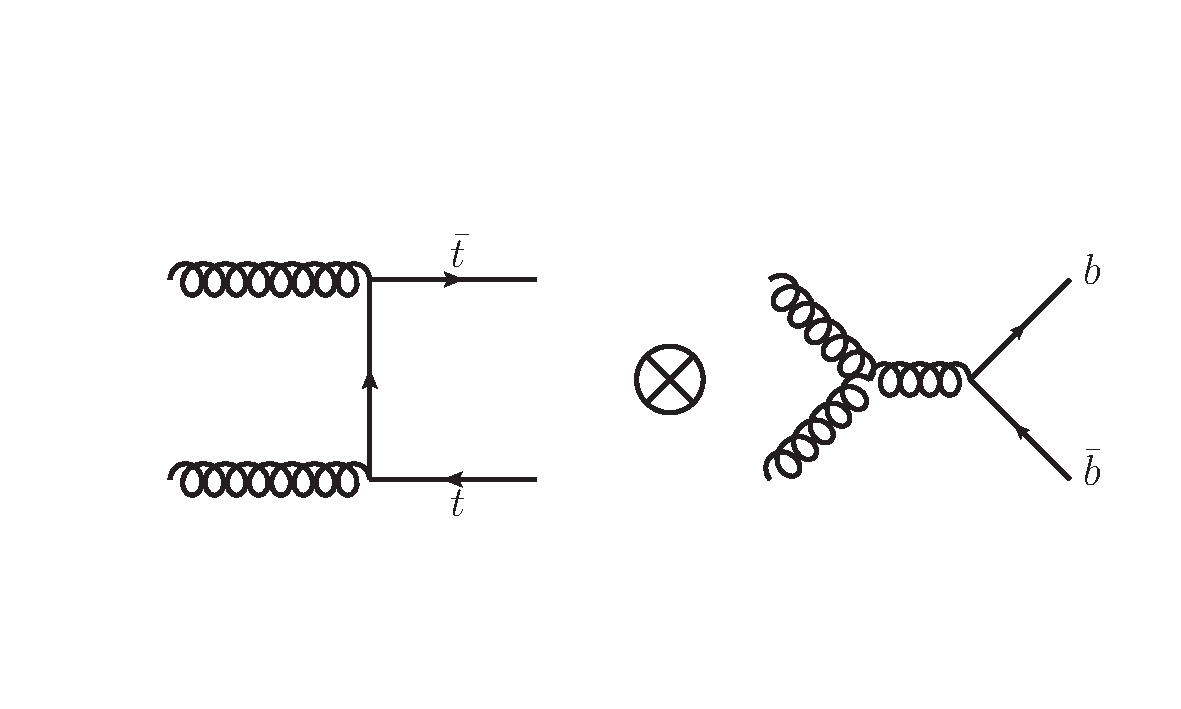
\includegraphics[width=0.9\textwidth]{figures/Datasamples/ttbb_MPI_good.pdf}
  \caption{}
  \label{fig:dat:ttb:fsr}
\end{subfigure}
\begin{subfigure}{0.5\textwidth}
  \centering
  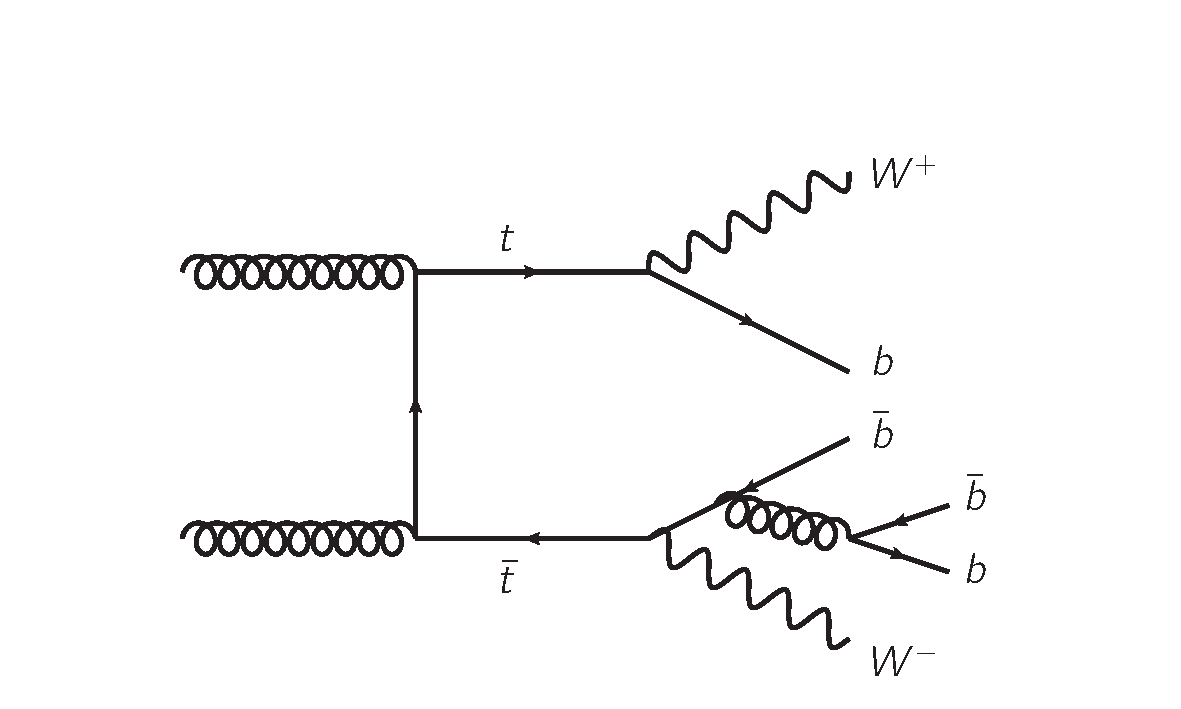
\includegraphics[width=0.9\textwidth]{figures/Datasamples/ttbb_FSR_good.pdf}
  \caption{}
  \label{fig:dat:ttb:mpi}
\end{subfigure}

\captionsetup{width=0.85\textwidth} \caption{\small (a) $b\bar{b}$ production from multiple parton interaction overlayed with a $t\bar{t}$ event from the hard scatter and (b) $g\to b\bar{b}$ from final-state radiation in a $\ttbar$ event.}
\label{fig:dat:ttb:mpifsr}
\end{figure}
\par The contribution of the various $t\bar{t}+\ge1b$ particle-jet topologies to the cross section is shown in figure \ref{fig:dat:ttb:xsecat}. The $t\bar{t}+b$ and $t\bar{t}+b\bar{b}$ are the two sub-categories that dominates the cross section; in those sub-categories the {\sc MG5$\_$aMC} samples and the {\sc Powheg-Box+Pythia} sample predict higher cross sections than {\sc SherpaOL}, with discrepancies that go up to $30\%$.  Some examples of normalised distributions of different relevant variables the two main sub-categories are shown in figure \ref{fig:dat:ttb:kincat}. The {\sc MG5$\_$aMC} samples and the {\sc Powheg-Box+Pythia} sample predict a softer spectrum for the leading extra $b$-jet in the $t\bar{t}+b$ sub-category compared to {\sc SherpaOL}, with differences up to $20\%$, as shown in figure \ref{fig:dat:ttb:bpt}. For the $\Delta R$ between the two leading b-jets in $t\bar{t}+b\bar{b}$ sub-category, shown in figure \ref{fig:dat:ttb:drbb}, the disagreements are smaller, reaching only $10\%$. 

\bfig[b!]
\centering
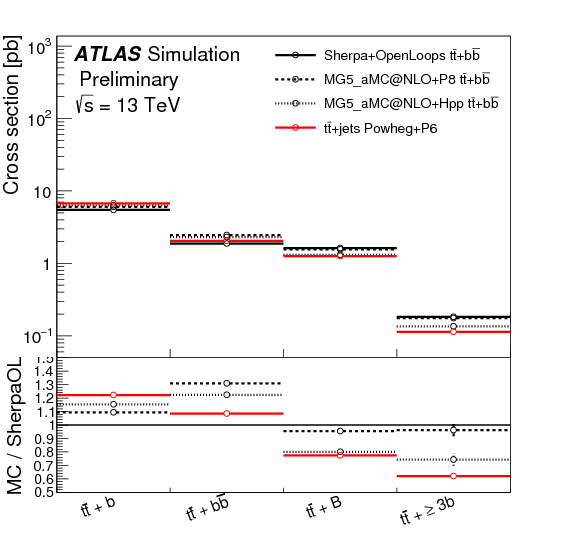
\includegraphics[width=0.5\textwidth]{figures/Datasamples/ttbbxsec2.png}
\captionsetup{width=0.85\textwidth} \caption{\small Cross section for different categories of $t\bar{t}+\ge1b$ events. The three 4FNS NLO samples are compared to the {\sc Powheg-Box+Pythia} $t\bar{t}$+jets sample.}
\label{fig:dat:ttb:xsecat}
\efig



\begin{figure}[t!]
\begin{subfigure}{0.5\textwidth}
  \centering
  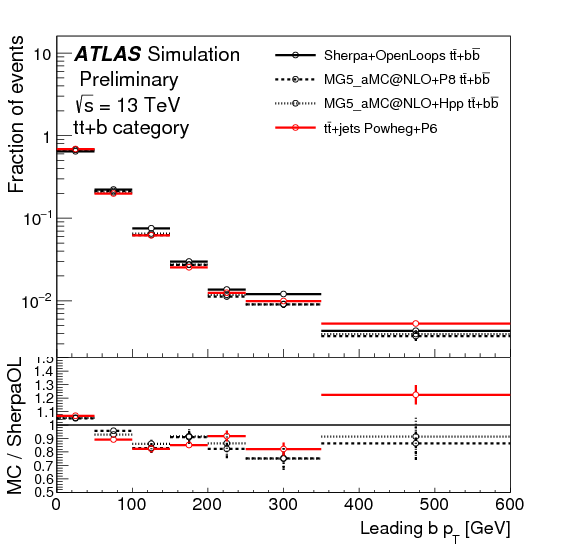
\includegraphics[width=0.9\textwidth]{figures/Datasamples/bpt2.png}
  \caption{}
  \label{fig:dat:ttb:bpt}
\end{subfigure}
\begin{subfigure}{0.5\textwidth}
  \centering
  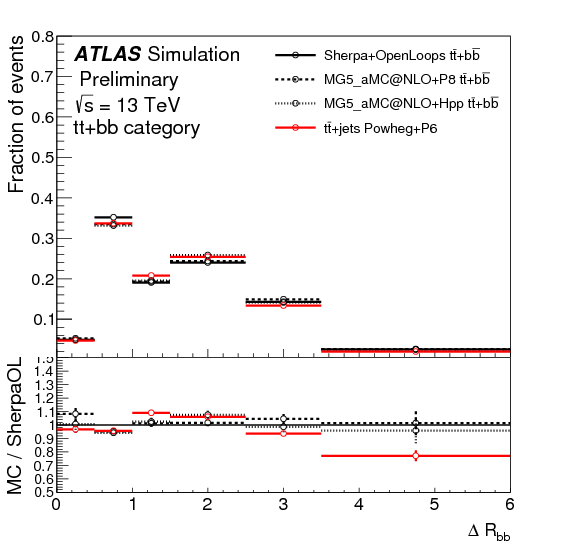
\includegraphics[width=0.9\textwidth]{figures/Datasamples/drbb2.png}
  \caption{}
  \label{fig:dat:ttb:drbb}
\end{subfigure}

\captionsetup{width=0.85\textwidth} \caption{\small (a) Transverse momentum of the leading extra $b$-jet in the $t\bar{t}+b$ sub-category and (b) $\Delta R$ between the two leading $b$-jets in the $t\bar{t}+b\bar{b}$ sub-category.}
\label{fig:dat:ttb:kincat}
\end{figure}

To improve the $t\bar{t}+\ge1b$ modelling in {\sc Powheg-Box+Pythia}, a reweighting procedure is applied to match the prediction from {\sc SherpaOL}.
The correction is performed by applying a kinematic reweighting separately in each of the $t\bar{t}+\ge1b$ sub-categories, such that the relative normalisation of the sub-categories and the kinematic distributions match the {\sc SherpaOL} prediction. In each sub-category, a two-dimensional reweighting based on the $\pt$ of the top quark and the $\pt$ of the $t\bar{t}$ system is performed. This is followed in the $t\bar{t}+b\bar{b}$ and $t\bar{t}+\ge3b$ sub-categories by a two-dimensional reweighting of the $\Delta R$ between the two leading $b$-jets and the $\pt$ of the system of the two leading $b$-jets; in the $t\bar{t}+B$ and $t\bar{t}+b$ sub-categories, the $B$ or $b$-jet $\pt$ and $\eta$ are used instead.
This reweighting improves the modelling of the rest of the variables, though some minor differences remain. The effect of the reweighting both on shape and normalisation is $<10\%$ (e.g. see figure \ref{fig:dat:ttbb:reweigting}). 
 As discussed in section \ref{chp:vlq:sec:syst}, the 4FNS NLO prediction from {\sc MG5$\_$aMC} will be used to assess systematic uncertainties. 
 
 \begin{figure}[htb!]
\begin{subfigure}{0.5\textwidth}
  \centering
  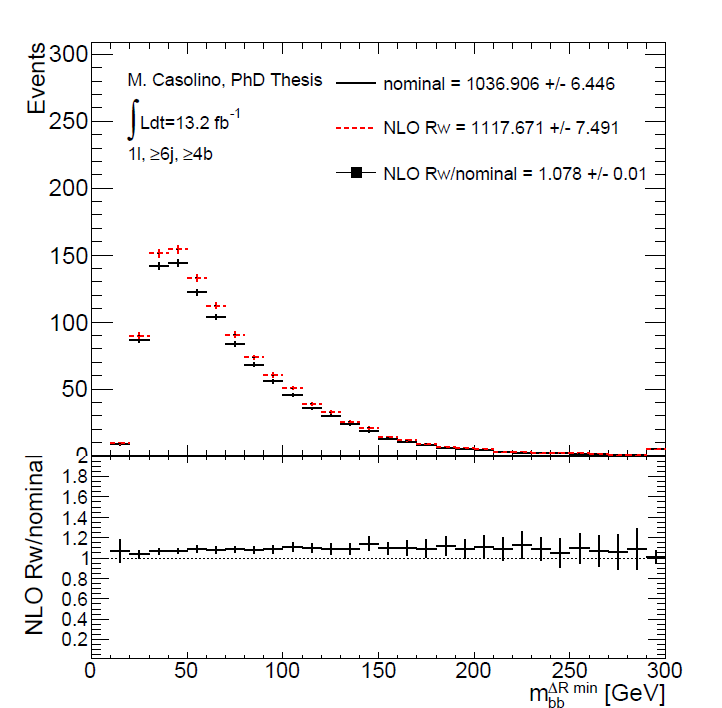
\includegraphics[width=0.9\textwidth]{figures/Datasamples/ttbb_mbb_mindR_c1l6ji4bi_.png}
  \caption{}
  \label{fig:dat:trf:regiontwob}
\end{subfigure}
\begin{subfigure}{0.5\textwidth}
  \centering
  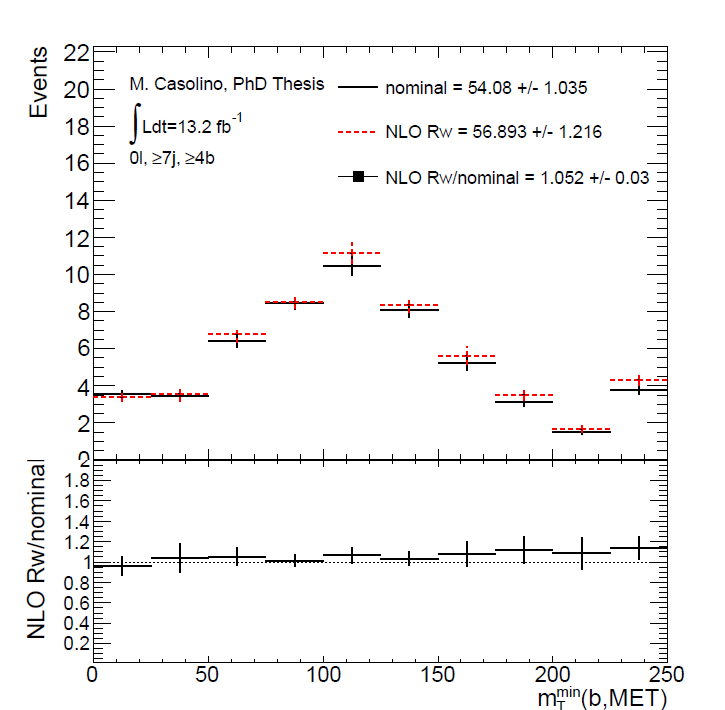
\includegraphics[width=0.9\textwidth]{figures/Datasamples/ttbb_mtbmin_zoom_c0l7ji4bi_.png}
  \caption{}
  \label{fig:dat:trf:regionfourb}
\end{subfigure}

\captionsetup{width=0.85\textwidth} \caption{\small (a) The mass of the $b\bar{b}$ pair with smallest $\Delta R$ distance, $m_{b\bar{b}}^{{\rm min}\Delta R}$ for events with one lepton at least six jets and at least four $b$-tags, and (b) the minimum transverse mass between \MET and any of the three leading $b$-tagged jets in the event, $m_{\rm T,min}^b$, for events with no lepton at least seven jets and at least four $b$-tags. In red the prediction obtained with the reweighting to {\sc SherpaOL} and in black the nominal prediction.}
\label{fig:dat:ttbb:reweigting}
\end{figure}

\subsubsection[$t\bar{t}+\ge 1c$]{\boldmath{$t\bar{t}+\ge 1c$}}
\label{sec:data:ttc}
In case of $t\bar{t}+\ge1c$ production, there is little guidance from theory or experiment on whether the parton shower provides a sufficiently accurate modelling of this process or whether a prediction with $t\bar{t}+c\bar{c}$ calculated in the matrix element is needed. Therefore, {\sc Powheg-Box+Pythia} is used for the $t\bar{t}+\ge1c$ prediction, with the possibility of applying as correction the  $t\bar{t}$ and top-quark $\pt$ NNLO reweighting or only the top-quark $\pt$ NNLO  reweighting. A novel simulation \cite{ATL-PHYS-PUB-2016-011} using {\sc MG5$\_$aMC} interfaced with {\sc Herwig++} to generate $t\bar{t}+c\bar{c}$ at NLO in 3FNS using the CT103f PDF set is used to assess systematic uncertainties for analyses particularly sensitive to this background as described in section \ref{sec:tth:systunc}.

\subsection[$W/Z$+jets production]{\boldmath{$W/Z$}+jets production}
The production of a single $W$ or $Z$ boson associated with additional jets is simulated using {\sc Sherpa} 2.2 for all analyses presented in this dissertation, except for the $t\bar{t}H$ search where a slightly older version, 2.1.1 was used. The matrix element calculation is performed using up to two partons at NLO and up to four parton at LO using {\sc Comix} and {\sc OpenLoops} and then merged with the {\sc Sherpa} parton shower using the MEPS@NLO prescription \cite{Hoeche:2012yf}. The PDF set used in the calculation is CT10 with a dedicated parton shower tuning developed for {\sc Sherpa}. Samples are generated separately for $W/Z$+light-jets, $W/Z+\ge1b$ and $W/Z+\ge1c$ using filters and then combined into the inclusive sample. Both $W$+jets and $Z$+jets processes are normalised to their respective NNLO theoretical cross sections calculated with {\sc Fewz} \cite{Anastasiou:2003ds}.

\subsection{Single top-quark production}
Samples of single top-quark production in $t$-channel are generated using the {\sc Powheg-Box} 2.0 generator that uses the 4FNS for the NLO matrix element calculations and the fixed four-flavour CT10f4 PDF set. Samples corresponding to the $s$-channel and $Wt$ production mechanisms are generated with {\sc Powheg-Box} 2.0 at NLO using the CT10 PDF set. For the $Wt$ samples, the ``diagram removal'' scheme \cite{Frixione:2005vw} is used to remove the overlap with $t\bar{t}$ production. The parton shower, hadronisation and the underlying event are modelled using {\sc Pythia} 6.425 with the CTEQ6L1 PDF set in combination with the P2012 UE tune. The single-top-quark samples are normalised to the approximate NNLO theoretical cross sections \cite{Kidonakis:2011wy,Kidonakis:2010ux,Kidonakis:2010tc}.\par
Higgs boson production in association with a single top quark is also considered. The $tHbj$ process is generated with {\sc MG5$\_$aMC} interfaced to {\sc Herwig++} with the UE-EE5 tune. The CT10 PDF set is used, and the renormalisation and factorisation scales are fixed to 75 \gev. The $tWH$ process is produced with the same generators and settings, but the renormalisation and factorisation scales are set to $H_{\rm T}/2$. The cross sections are calculated at NLO \cite{Demartin:2015uha}.

\subsection{Diboson production}
Samples of $WW/WZ/ZZ$+jets events are generated with {\sc Sherpa} 2.1.1 using the CT10 PDF set and include processes containing up to four electroweak vertices. The matrix-element includes zero additional partons at NLO and up to three partons at LO using the same matching procedure between matrix element and parton shower as for the $W/Z$+jets samples. A requirement of a leptonic decay of at least one boson is applied at generation level. All diboson samples are normalised to their NLO theoretical cross sections provided by {\sc Sherpa}.

\subsection[$t\bar{t}V$ production]{\boldmath{$t\bar{t}V$} production}
Samples of $t\bar{t}V$ events are generated with {\sc MG5$\_$aMC} 2.3.2, using LO matrix elements including up to one parton for $t\bar{t}\gamma^{*}/Z,\gamma^{*}/Z\to \ell^{+}\ell^{-}$ with $\ell=e$, $\mu$, $\tau$ and two partons for $t\bar{t}W$ and $t\bar{t}Z,Z\to \nu\bar{\nu}$. For all samples showering is performed using {\sc Pythia} 8.210 and the A14 UE tune, using  the NNPDF2.3LO PDF set. The $t\bar{t}V$ samples are normalised to their NLO cross sections \cite{ttV1,ttV2}.

\subsection{Multijet production}
\label{chp:sec:sigbkg:qcd}
Multijet events can enter the selected data sample through several production and misreconstruction mechanisms. In the case of non-prompt or fake electrons, these include contributions from semileptonic decays of $b$- and $c$-quarks, photon conversions and jets with large electromagnetic energy (from hadronisation to giving an energetic $\pi^{0}$ or from early showering in the calorimeter).  Non-prompt or fake muons can originate from semileptonic decays of $b$- and $c$-hadrons, from charged-hadron decays in the tracking volume or in hadronic showers, or from punch-through particles emerging from high-energy hadronic showers. While the probability of reconstructing a lepton from a ``fake'' source in a multijet event is very low,  multijet events are characterised by a cross section several orders of magnitude larger than typical sources of prompt leptons ($W$ and $Z$ bosons).\par
Since this background is very difficult to model accurately with a MC simulation, a data-driven method, referred to as Matrix Method \cite{Aad:2010ey} (MM), is used to estimate the expected number of multijet events in the final selection sample. The MM relies on the difference in the lepton identification efficiency between real and ``fake'' leptons. It uses two samples: a ``tight'' sample, which corresponds to the final event selection, and a ``loose'' sample, which is obtained from the tight sample by relaxing some of the identification and isolation requirements (see sections \ref{chp:obj:sec:ele} and \ref{chp:obj:sec:muon}). Due to the relaxation of the selection criteria, the loose sample contains a higher fraction of fake leptons. The number of selected events in each sample ($N_{\rm loose}$ and $N_{\rm tight}$) are given by the sum of events containing real and fake leptons: 

\be
N_{\rm loose}=N^{\rm real}_{\rm loose}+N^{\rm fake}_{\rm loose},
\label{sec:bkq:eq:looselep}
\ee
\be
N_{\rm tight}=\epsilon^{\rm real}\cdot N^{\rm real}_{\rm loose}+\epsilon^{\rm fake}\cdot N^{\rm fake}_{\rm tight},
\label{sec:bkq:eq:tightlep}
\ee

\noindent where $\epsilon^{\rm real}$ ($\epsilon^{\rm fake}$) represents the probability for a real (fake) lepton satisfying the loose criteria to also satisfy the tight criteria, and both are measured in data control samples. An estimate for the number of events with fake leptons in the tight sample is obtained by solving the above system of equations:
\be
N_{\rm tight}^{\rm fake}=\frac{\epsilon^{\rm fake}}{\epsilon^{\rm real}-\epsilon^{\rm fake}}\cdot (\epsilon^{\rm real} \cdot N_{\rm loose} - N_{\rm tight}).
\label{chp:data:eq:fakes}
\ee
As shown in equation \ref{chp:data:eq:fakes}, the power of the method resides in having sufficiently different efficiencies for the real and fake leptons. 
The efficiencies $\epsilon^{\rm real}$ and $\epsilon^{\rm fake}$ depend on lepton kinematics and event characteristics, such as the number of jets or $b$-jets. To correctly account for this, an event weight is computed from the efficiencies, which are parametrised as a function of the various object kinematics:

\be
w_{i}=\frac{\epsilon^{\rm fake}}{\epsilon^{\rm real}-\epsilon^{\rm fake}}\cdot (\epsilon^{\rm real}-\delta_{i})
\ee
where $\delta_{i}$ equals unity if the loose event $i$ passes the tight event selection and 0 otherwise. The background estimate in a given bin of the final observable is given by the sum of $w_{i}$ over all events in that bin.


The efficiencies $\epsilon^{\rm real}$ and $\epsilon^{\rm fake}$ are extracted from data in specific control regions designed to increase the fraction of real and fake leptons. For $\epsilon^{\rm real}$  the tag and probe method is employed to extract a very pure sample of prompt isolated leptons from $Z\to \ell^{+}\ell^{-}$ decays. The average $\epsilon^{\rm real}$ is $\sim0.89$ ($\sim0.93$) for electrons (muons). To measure $\epsilon^{\rm fake}$, samples enriched in multijet background are selected by requiring one loose lepton, one $b$-jet, low \MET, low transverse mass between the lepton and the \MET,\footnote{See equation \ref{sec:vlq:eq:mtw} for the definition.} and high impact parameter significance for the track (required only for muons). The average $\epsilon^{\rm fake}$ value is 0.17 (0.43) for electrons (muons).


\subsection{Signal modelling}
\subsubsection[$t\bar{t}H$ production]{\boldmath{$t\bar{t}H$} production}
The $t\bar{t}H$ signal process is modelled at NLO using {\sc MG5$\_$aMC} 2.3.2, interfaced to the {\sc Pythia} 8.210 parton shower using the A14 UE tune. The NNPDF3.0NLO PDF set is used, and the factorisation and renormalisation scales are set to $\mu_{F} = \mu_{R} = H_{\rm T}/2$, where $H_{\rm T}$ is defined as the scalar sum of the transverse energies of all final state particles. The top quarks are decayed using {\sc MadSpin} \cite{madspin}, preserving all spin correlations. The sample is normalised to the NLO cross section \cite{ttH1,ttH2,ttH3,Yu:2014cka,Frixione:2015zaa}. All decay modes are considered and the branching ratios are calculated using {\sc Hdecay} \cite{hdecay}.

\subsubsection{Vector-like quark pair production }
Samples of simulated $T\bar{T}$ events are generated with the LO generator {\sc Protos} 2.2 using the NNPDF2.3 LO PDF set and processed through {\sc Pythia} 8.186 for parton showering and fragmentation using the A14 UE tune. The vector-like quarks are forced to decay with a branching ratio of $1/3$ to each of the three modes ($W$, $Z$, $H$). Events are reweighted using generator-level information to obtain any arbitrary sets of branching ratios consistent with the three decay modes summing to unity. Samples are generated assuming singlet couplings and for heavy-quark masses between 350 $\gev$ and 1500 $\gev$ in steps of 50 \gev. Additional samples are produced for a few mass points assuming doublet couplings, in order to confirm that kinematic differences arising from the different chirality of singlet and doublet couplings, after reweighting the singlet and doublet samples to the same branching ratios, have negligible impact on this analysis. The  $T\bar{T}$ samples are normalised using the theoretical cross section computed using {\sc Top++} 2.0 at NNLO including resummation of NNLL soft-gluon terms, and using the MSTW 2008 NNLO PDF set.
\subsubsection{Four-top-quark production}
Samples of simulated four-top-quark events for the three production mechanisms discussed in section \ref{sec:theo:fourtops} are generated at LO with the {\sc MG5$\_$aMC} generator (the versions used are 2.2.2, 2.2.3 and 1.5.14 for SM, EFT and 2UED/RPP, respectively) and the NNPDF2.3 LO PDF set, interfaced to {\sc Pythia} 8 (the versions used are 8.186, 8.205 and 8.186 for SM, EFT and 2UED/RPP, respectively) and the A14 tune. The SM $t\bar{t}t\bar{t}$ sample is normalised to a cross section of 9.2 fb (computed at NLO with {\sc MG5$\_$aMC}), while the EFT $t\bar{t}t\bar{t}$ sample is normalised assuming $|C_{4t}/\Lambda^{2}|=4\pi$ $\tev^{-2}$, which yields a cross section of 928 fb. In the case of the 2UED/RPP model, samples are generated for four different values of $m_{KK}$ (1000 to 1800 $\gev$ in steps of 200 $\gev$) and the {\sc Bridge} \cite{Meade:2007js} generator is used to decay the pair-produced excitations from tier (1,1) generated by {\sc MG5$\_$aMC}.

\subsubsection{Associated production of heavy Higgs bosons}
Samples of simulated $b\bar{b}H(\to t\bar{t})$ and $t\bar{t}H(\to t\bar{t})$ events are generated assuming a Type-II 2HDM model using the {\sc MG5$\_$aMC} 2.3.3 generator, interfaced to {\sc Pythia} 8.210 and the A14 tune. The matrix-element calculation is performed at LO in 4FNS and the corresponding 4FNS CTEQ6L1 PDF set is used. Spin correlations are taken into account in the decays of top quarks and $W$ bosons. Samples are generated for heavy Higgs-boson masses between 400 $\gev$ and 1000 $\gev$ in steps of 100 \gev. These samples can also be used to model $b\bar{b}A(\to t\bar{t})$ and $t\bar{t}A(\to t\bar{t})$ production, as generator level studies showed no significant differences in the kinematics of the decay products for processes involving the production of a CP-even or CP-odd Higgs boson of the same mass. The $tbH^{\pm}(\to tb)$ samples are generated at NLO using {\sc MG5$\_$aMC} 2.2.2 with the NNPDF2.3 PDF set, interfaced to {\sc Pythia} 8.212 with the A14 tune. A Type-II 2HDM model is assumed. The width of the charged Higgs boson has been set to zero. Samples are generated for charged Higgs boson masses between 200 \gev and 2000 \gev.\par
All samples are normalised to a reference cross section times branching ratio of 1 pb. For the interpretation of results, cross sections and branching ratios are computed separately for Type-I and Type-II 2HDMs, as a function of heavy Higgs boson mass, $\tan \beta$ and $\cos(\beta - \alpha)$. In the case of $b\bar{b}H(\to t\bar{t})$ and $t\bar{t}H(\to t\bar{t})$ production, the predictions are obtained using the codes {\sc SusHi} 1.5.0 \cite{Harlander:2012pb}, which implements calculations from references \cite{Harlander:2002wh,Harlander:2003ai,Aglietti:2004nj,Bonciani:2010ms,Harlander:2005rq}, and {\sc 2Hdmc} 1.7.0 \cite{Eriksson:2009ws}. The $t\bar{t}H(\to t\bar{t})$ cross sections are computed at NLO, whereas the $b\bar{b}H(\to t\bar{t})$ cross sections are obtained from the so-called ``Santander matching" of NLO cross sections in 4FNS and NNLO cross sections in 5FNS \cite{Harlander:2011aa}. Similarly, the $tbH^{\pm}(\to tb)$ cross sections are obtained using the ``Santander matching" of 4FNS NLO and 5FNS NNLO cross sections \cite{Degrande:2015vpa,Flechl:2014wfa,Heinemeyer:2013tqa,Berger:2003sm}. The charged Higgs boson branching ratios are also obtained using {\sc 2Hdmc}.

